\documentclass[../../../../main.tex]{subfiles}

\begin{document}

\section*{京大理科 数学 1974 表紙・配点・概略}

\begin{itemize}
    \item 所要時間: 120分 / 150分
\end{itemize}

\subsection*{各問のメモ・解答概要}
\begin{enumerate}
    \item 3点 $A, B, C$ が単位円上にあるとき、重心が原点ならば外心と一致し正三角形となることを示す。[解2]では $\cos^2\gamma + \sin^2\gamma = 1$ を用いて $\beta - \alpha$, $\gamma - \alpha$ の差を計算する。
    \item 水槽の底からの水深 $h = 10 - vt$ を微分方程式より求め、水量 $V(t) = \pi \left( 100vt - \frac{1}{3}v^3 t^3 \right)$ および流出速度 $k = \pi v (100 - v^2 t^2)$ を算出する。
    \item 4次関数 $f_q(x) = x^4 - 6p^2 x^2 - 8q^3 x$ の導関数と極値・凹凸の増減表を提示し、$p > q$ の場合は矛盾が生じ、$p \le q$ のとき $A$ が右のくぼみに落ちることから $\min q = p$ を導く。
    \item 多項式 $F(x) = (ax+b)g(x)$ とおき、最高次および次数の比較から $b=0, a=\frac{1}{n+1}$ を得て、微分方程式 $\frac{n}{x}dx = \frac{1}{y}dy$ を解くことで $g(x) = x^n$, $F(x) = \frac{1}{n+1}x^{n+1}$ を求める。
    \item (i) 不等式をみたす整数解の個数が有限個であることを示し、(ロ)(ハ) では $\bmod 4$ の条件等から $n^2 = 4m+1$ に限られることを用いて最大値 $(n, m) = (17, 72)$ を求める。
\end{enumerate}

\newpage

\section*{第1問}

\noindent
[\textbf{解}] 3点 $A(\cos\alpha, \sin\alpha), B(\cos\beta, \sin\beta), C(\cos\gamma, \sin\gamma)$ を頂点とする $\Delta ABC$ を考える. この外心は $(0,0)$ で, 題意から重心も $(0,0)$ である.

外心と重心が一致するのは正三角形なので, $\Delta ABC$ は正三角形.

(以上により $0 \le \alpha < \beta < \gamma \le 2\pi$ を用いた).

従って
\[
\beta - \alpha = \gamma - \beta = \frac{2\pi}{3} \quad /\!/
\]

\bigskip
\noindent
[\textbf{解2}]
$\cos^2\gamma + \sin^2\gamma = 1$ に代入
\[
2 + 2\cos(\beta - \alpha) = 1
\]
\[
\cos(\beta - \alpha) = -\frac{1}{2}
\]
\[
\therefore \beta - \alpha = \frac{2}{3}\pi, \, \frac{4}{3}\pi
\]
同様にして
\[
\gamma - \alpha = \frac{2}{3}\pi, \, \frac{4}{3}\pi
\]
以上と $0 \le \alpha < \beta < \gamma < 2\pi$ から
\[
\beta - \alpha = \frac{2}{3}\pi, \quad \gamma - \alpha = \frac{4}{3}\pi
\]
\[
\therefore \gamma - \beta = \frac{2}{3}\pi \quad /\!/
\]

\newpage

\section*{第2問}

\begin{center}
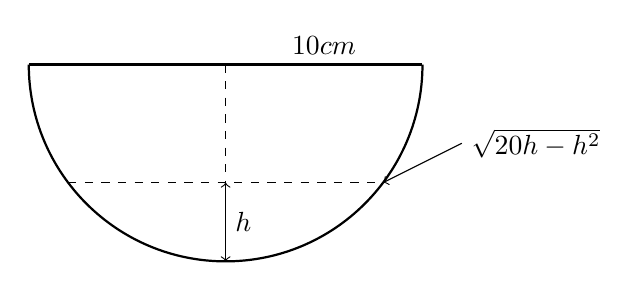
\begin{tikzpicture}[scale=0.25]
    \draw[thick] (-10,0) arc (180:360:10);
    \draw[thick] (-10,0) -- (10,0);
    \draw[dashed] (0,0) -- (10,0);
    \node[above] at (5,0) {$10\text{ cm}$};
    \draw[dashed] (-8,-6) -- (8,-6);
    \draw[dashed] (0,0) -- (0,-10);
    \draw[<-] (8,-6) -- (12,-4) node[right] {$\sqrt{20h-h^2}$};
    \draw[<->] (0,-10) -- (0,-6) node[midway,right] {$h$};
\end{tikzpicture}
\end{center}

\noindent
[\textbf{解}] 時刻 $t$ での水面の面積 $S$, 水深を $h$ とすると, 水の流出速度 $k$ として
\begin{equation}
-k = S \frac{dh}{dt} \quad \cdots \text{①}
\end{equation}
ここで,
\begin{equation}
S = \pi (20h - h^2) \quad \cdots \text{②}
\end{equation}
又, 題意から,
\[
-v = \frac{dh}{dt}
\]
であり, 両辺積分して, $t=0$ で $h=10$ より,
\begin{equation}
h = 10 - vt \quad \cdots \text{③}
\end{equation}

\noindent
(1) 題意の水量 $V(t)$ とすると,
\[
V(t) = \pi \int_0^{vt} (100 - x^2) dx = \pi \left[ 100x - \frac{1}{3}x^3 \right]_0^{vt} = \pi \left( 100vt - \frac{1}{3}v^3 t^3 \right) \quad /\!/
\]

\noindent
(2) ①, ②, ③から
\[
k = S v = \pi v (20-h) h = \pi v (10+vt)(10-vt) = \pi v (100 - v^2 t^2) \quad /\!/
\]

\newpage

\section*{第3問}

\noindent
[\textbf{解}] $f_q(x) = x^4 - 6p^2 x^2 - 8q^3 x$ とおく. ($p > 0, q \ge 0$)

$f_q'(x) = 4x^3 - 12p^2 x - 8q^3$ だから, $q=0$ の時, 下表を得る

\begin{center}
\begin{tabular}{c|c|c|c|c|c|c|c}
$x$ & $\dots$ & $-\sqrt{3}p$ & $\dots$ & $0$ & $\dots$ & $\sqrt{3}p$ & $\dots$ \\ \hline
$f'$ & $-$ & $0$ & $+$ & $0$ & $-$ & $0$ & $+$ \\ \hline
$f$ & $\searrow$ & & $\nearrow$ & & $\searrow$ & & $\nearrow$
\end{tabular}
\end{center}

\noindent
従って, $A$ の $x$ 座標は $-\sqrt{3}p \; (\equiv x_0)$ である. 又, $f_q''(x) = 12(x^2 - p^2)$ から下表を得る

\begin{center}
\begin{tabular}{c|c|c|c|c|c}
$x$ & $\dots$ & $-p$ & $\dots$ & $p$ & $\dots$ \\ \hline
$f''$ & $+$ & $0$ & $-$ & $0$ & $+$ \\ \hline
$f'$ & $\nearrow$ & 8($p^3-q^3$) & $\searrow$ & 負 & $\nearrow$
\end{tabular}
\end{center}

\noindent
従って $q$ の値により下表をえる

\bigskip
\noindent
$1^\circ$ $p > q$ の時

$f_q'(-p) > 0$ から, $f_q'(x) = 0$ となる $x$ が 3つある ($\alpha < \beta < \gamma$ とする)

\begin{center}
\begin{tabular}{c|c|c|c|c|c|c|c}
$x$ & $\dots$ & $\alpha$ & $\dots$ & $\beta$ & $\dots$ & $\gamma$ & $\dots$ \\ \hline
$f'$ & $-$ & $0$ & $+$ & $0$ & $-$ & $0$ & $+$ \\ \hline
$f$ & $\searrow$ & & $\nearrow$ & & $\searrow$ & & $\nearrow$
\end{tabular}
\end{center}

\noindent
この時 $A$ が右のくぼみに落ちるのは, $\beta \le -\sqrt{3}p \le \gamma$ の時である. $\quad \cdots \text{①}$

\noindent
しかし, 本から $-p < \beta$ であり, 又 $p > 0$ から $-\sqrt{3}p < -p$ だから ①がみたされることはなく, 矛盾.

\bigskip
\noindent
$2^\circ$ $p \le q$ の時

$f_q'(-p) \le 0$ から, $f_q'(x) = 0$ となる $x$ が唯一存在する ($\alpha$ とする)

\begin{center}
\begin{tabular}{c|c|c|c}
$x$ & $\dots$ & $\alpha$ & $\dots$ \\ \hline
$f'$ & $-$ & $0$ & $+$ \\ \hline
$f$ & $\searrow$ & & $\nearrow$
\end{tabular}
\end{center}

\noindent
よって, $A$ が右のくぼみに落ちるのは $-\sqrt{3}p \le \alpha$ つまり $f_q'(-\sqrt{3}p) \le 0$ の時,
\[
f_q'(-\sqrt{3}p) = -8q^3 \le 0 \quad \therefore q \ge 0
\]
したがって, $0 < p$ から $p \le q$ の時, $A$ が右のくぼみにおちる.

\noindent
以上 $1^\circ, 2^\circ$ から求める $\min q = p$ である.

\begin{center}
\begin{tikzpicture}[scale=0.8]
    \draw[->] (-3,0) -- (3,0) node[right] {$x$};
    \draw[->] (0,-4) -- (0,2) node[above] {$y$};
    \draw[domain=-2.1:2.1,smooth,variable=\x,thick,blue] plot ({\x}, {0.3*(\x+1.5)*(\x+1.5)*(\x-1.8)});
    \fill (-2,0) circle (1.5pt) node[below] {$-\sqrt{3}p$};
    \fill (-1.5,0) circle (1.5pt) node[below] {$-p$};
    \fill (1.8,0) circle (1.5pt) node[below] {$2p$};
    \node[below right] at (0,0) {$O$};
\end{tikzpicture}
\end{center}
\noindent
$\left[\text{この時, } f'(x) = 4(x^3 - 3p^2 x - 2p^3) = 4(x+p)^2 (x-2p) \text{ となり,}\right]$ $\Rightarrow$ 予想通り!

\newpage

\section*{第4問}

\noindent
[\textbf{解}] (イ)から $F(x)$ は $m+1$ 次だから, $a \neq 0, a, b \in \mathbb{R}$ として
\begin{equation}
F(x) = (ax+b) g(x) \quad \cdots \text{①}
\end{equation}
とおける. ((ロ)) 両辺微分して
\begin{equation}
g(x) = a g(x) + (ax+b) g'(x) \quad \cdots \text{②}
\end{equation}

\noindent
又, (ハ)から, $g(x) = x^n + a_{n-1} x^{n-1} + \dots$ となるから $g'(x) = n x^{n-1} + (n-1) a_{n-1} x^{n-2} + \dots$ となる. ②において $x^n, x^{n-1}$ の項を比較して
\begin{equation}
\begin{cases}
x^n = a x^n + a n x^n \quad \cdots \text{③} \\
0 = 0 + b n x^{n-1} \quad \cdots \text{④}
\end{cases}
\end{equation}
$n > 0$ と ③, ④ から, $b = 0, \, a = \frac{1}{1+n}$ となるので $g(x) = y$ として ②に代入
\[
\frac{n}{1+n} y = \frac{1}{n+1} x \frac{dy}{dx}
\]
\[
\frac{n}{x} dx = \frac{1}{y} dy
\]
両辺積分して
\[
n \log x + C_1 = \log y \quad (C_1: \text{定数})
\]
\[
y = e^{C_1} x^n
\]
$g(x)$ の $x^n$ の係数は 1 だから $e^{C_1} = 1$ となり
\[
g(x) = x^n \quad /\!/
\]
①から
\[
F(x) = \frac{1}{n+1} x^{n+1} \quad /\!/
\]

\newpage

\section*{第5問}

\noindent
[\textbf{解}] (i) $\frac{a}{\sqrt{m}} + \frac{b}{m}$ は $m$ について単調減少で ($\because m, a, b > 0$)
$m \to \infty$ で $0$ に収束し, $m=1$ で $a+b$ をとるから,

\bigskip
\noindent
$1^\circ$ $a+b < 1$ の時,
\[
4m < n^2 < 4m + \frac{a}{\sqrt{m}} + \frac{b}{m} < 4m+1
\]
となり, これが解答を持つとすると $4m$ と $4m+1$ の間に整数が存在することになり, 矛盾. よってこの時与不等式は解なし.

\bigskip
\noindent
$2^\circ$ $a+b \ge 1$ の時,
\[
\frac{a}{\sqrt{m_0}} + \frac{b}{m_0} \ge 1 > \frac{a}{\sqrt{m_0+1}} + \frac{b}{m_0+1}
\]
をみたす $m_0 \in \mathbb{N}$ が存在する. $m \ge m_0+1$ の時, $1^\circ$ と同じく与不等式は解なし. したがって解答があるのは $1 \le m \le m_0$ の時. さらにこの時,
\[
4m < N < 4m + \frac{a}{\sqrt{m}} + \frac{b}{m}
\]
をみたす $N \in \mathbb{N}$ は $\left[ \frac{a}{\sqrt{m}} + \frac{b}{m} \right]$ であるから, 全ての $N$ に $n \in \mathbb{Z}$ が 2つずつ対応していたとしても, $n$ は $2 \left[ \frac{a}{\sqrt{m}} + \frac{b}{m} \right]$ 個である. 以上から, 解は多くとも
\[
\sum_{m=1}^{m_0} 2 \left[ \frac{a}{\sqrt{m}} + \frac{b}{m} \right]
\]
であり, これは有限の値をとる.

\noindent
以上 $1^\circ, 2^\circ$ から示された. $\quad /\!/$

\bigskip
\noindent
(ロ) $4m < n^2 < 4m + \frac{8}{\sqrt{m}} + \frac{9}{m}$ ($m \ge 9$). $\quad \cdots \text{①}$

\noindent
$f(x) = \frac{8}{\sqrt{x}} + \frac{9}{x}$ とおく. $f'(x) = -\frac{4}{x\sqrt{x}} - \frac{9}{x^2} = -\frac{1}{x^2}(4\sqrt{x}+9)$ は $x \ge 9$ の時負の値をとるから, $x \ge 9$ で $f(x)$ は単調減少. これと $f(9) = \frac{11}{3}$ だから, $m \ge 9$ の時, $f(m) \le \frac{11}{3}$ である. 従って ①をみたす $n^2$ は
\[
n^2 = 4m+1, \, 4m+2, \, 4m+3
\]
に限られる. ここで, $\bmod 4$ で考えると, $n^2 \equiv 0, 1$ だから, 適するものは $n^2 = 4m+1$ に限られる.

\bigskip
\noindent
(ハ) $n>0$ の時を考えれば良く, この時 (ロ)から $n = \sqrt{4m+1}$, つまり $n$ が最大の時 $m$ が最大である. まず, $n^2 = 4m+1$ が解であるには
\[
1 < \frac{8}{\sqrt{m}} + \frac{9}{m}
\]
\[
\Leftrightarrow (m-9)^2 < 64m \quad (\because m \ge 9)
\]
が必要. これを解いて, $19 \le m \le 80$ とあわせて
\[
9 \le m \le 80 \quad \cdots \text{②}
\]
だから
\[
0 < 37 \le 4m+1 \le 321 \quad \cdots \text{③}
\]
であり, $36 < 37 \le 49$ から $6 < \sqrt{37} < 7$, $289 < 321 < 324$ から $17 < \sqrt{321} < 18$
なので, ③の両辺 $\sqrt{}$ をとって, $n \in \mathbb{N}$ から
\[
7 \le n \le 17
\]
従って $n=17$ をみたす $m$ があれば, これが求める値で, $n^2 = 4m+1$ を解いて計算すると $(n, m) = (17, 72)$ が求めるものである. $\quad /\!/$

\end{document}
